\section{Overview}
\label{sec:overview}

We start with an overview of our approach to
explaining (static) type errors using \emph{witnesses}
that (dynamically) show how the program goes wrong.
%
We illustrate why generating suitable inputs
to functions is tricky in the absence of type
information.
%
Then we describe our solution to the problem
and highlight the similarity to static type
inference,
%
Finally, we demonstrate our visualization of
the synthesized witnesses.

\subsection{Generating Witnesses}
\label{sec:generating-witnesses}
Our goal is to find concrete values
that demonstrate how a program ``goes wrong''.

\paragraph{Problem: Which inputs are bad?}
%
One approach is to randomly generate input values and
use them to execute the program until we find one that
causes the program to go wrong.
%
Unfortunately, this approach quickly runs aground.
Recall the erroneous @fac@ function from Figure~\ref{fig:factorial}.
%~\S~\ref{sec:introduction}:
%
% \begin{code}
  % let rec fac n =
    % if n <= 0 then
      % true
    % else
      % n * fac (n-1)
% \end{code}
% \ES{having two copies of \texttt{fac} seems silly, but the back-reference across a page boundary is no good either...}
%
What \emph{types} of inputs should we test @fac@ with?
%
Values of type @int@ are fair game, but values of type, say,
@string@ or @int list@ will cause the program to go wrong
in an \emph{irrelevant} manner.
%
Concretely, we want to avoid testing @fac@ with any type other
than @int@ because any other type would cause @fac@ to get stuck
immediately in the @n <= 0@ test.

\paragraph{Solution: Don't generate inputs until forced.}
Our solution is to avoid generating a concrete value for the input at
all, until we can be sure of its type.
%
The intuition is that we want to be as lenient as possible in our tests,
so we make no assumptions about types until it becomes clear from the
context what type an input must have.
%
This is actually quite similar in spirit to type inference.

To defer input generation, we borrow the notion of a ``hole'' from
SmallCheck~\cite{Runciman2008-ka}.
%
A hole --- written \vhole{\thole} --- is a \emph{placeholder} for a
value \ehole of some unknown type \thole.
%
We leave all inputs as uninstantiated holes until they are demanded by
the program, \eg due to a primitive operation like the @<=@ test.

\paragraph{Narrowing Input Types}
Primitive operations, data construction, and case-analysis \emph{narrow}
the types of values.
%
For concrete values this amounts to a runtime type check, we ensure that
the value has a type compatible with the expected type.
%
For holes, this means we now know the type it should
have (or in the case of compound data we know \emph{more} about the
type) so we can instantiate the hole with a value.
%
The value may itself contain more holes, corresponding to components
whose type we still do not know.
%
Consider the @fst@ function:
%
\begin{code}
  let fst p = match p with
    (a, b) -> a
\end{code}
%
The case analysis tells us that @p@ must be a pair, but it says
\emph{nothing} about the contents of the pair.
%
Thus, upon reaching the case-analysis we would generate a pair
containing fresh holes for the @fst@ and @snd@ component.
%
Notice the similarity between instantiation of type variables and
instantiation of holes.
%
We can compute an approximate type for @fst@ by approximating the types
of the (instantiated) input and output, which would give us:
%
\begin{mcode}
  fst : ($\thole_1$ * $\thole_2$) -> $\thole_1$
\end{mcode}
%
We call this type approximate because we only see a single path through
the program, and thus will miss narrowing points that only occur in
other paths.

Returning to @fac@, given a hole as input we will narrow the hole
to an @int@ upon reaching the @<=@ test.
%
At this point we choose a
random @int@\footnote{With standard heuristics~\cite{Claessen2000-lj} to favor small values.}
for the instantiation and
concrete execution takes over entirely, leading us to the expected crash
in the multiplication.

\paragraph{Witness Generality}
We show in \S~\ref{sec:soundness} that our lazy instantiation of holes
produces \emph{general witnesses}.
%
That is, we show that if ``executing''
a function with a hole as input causes the
function to ``go wrong'', then there is
\emph{no possible} type for the function.
%
In other words, for \emph{any} types you might
assign to the function's inputs, there exist values
that will cause the function to go wrong.

\paragraph{Problem: How many inputs does a function take?}
%
There is another wrinkle, though; how did we know
that @fac@ takes a single argument instead of two
(or none)?
%
It is clear, syntactically, that @fac@ takes \emph{at least} one
argument, but in a higher-order language with currying, syntax can be
deceiving.
%
Consider the following definition:
%
\begin{code}
  let incAllByOne = List.map (+ 1)
\end{code}
%
Is @incAllByOne@ a function?
%
If so, how many arguments does it take?
%
The \ocaml\ compiler deduces that @incAllByOne@ takes a single argument
because the \emph{type} of \hbox{@List.map@} says it takes two arguments, and it is
partially applied to @(+ 1)@.
%
As we are dealing with ill-typed programs we do not have the luxury of
typing information.

\paragraph{Solution: Search for saturated application.}
We solve this problem by deducing the number of arguments
via an iterative process. We add arguments one-by-one
until we reach a \emph{saturated} application, \ie\
until evaluating the application returns a value
other than a lambda.

\subsection{Visualizing Witnesses}
\label{sec:visual-witness}
We have described how to reliably find witnesses to type errors in \ocaml,
but this does not fully address our original goal --- to \emph{explain}
the errors.
%
Having identified an input vector that triggers a crash, a common next
step is to step through the program with a \emph{debugger} to observe
how the program evolves.
%
The existing debuggers and interpreters for \ocaml\ assume a type-correct
program, so unfortunately we cannot use them off-the-shelf.
%
Instead we extend our search for witnesses to produce an execution
trace.

\paragraph{Reduction Graph}
Our trace takes the form of a reduction graph, which records small-step
reductions in the context in which they occur.
%
% These graphs have two types of edges:
% %
% (1) ``steps-to'' edges that capture the small-step transition between
% two terms, and
% %
% (2) ``sub-term'' edges that capture the containment relation between two
% terms.
%
For example, evaluating the expression @1+2+3@ would produce the
graph in Figure~\ref{fig:simple-reduction-hi}.
%
\begin{figure}[t]
  \centering
  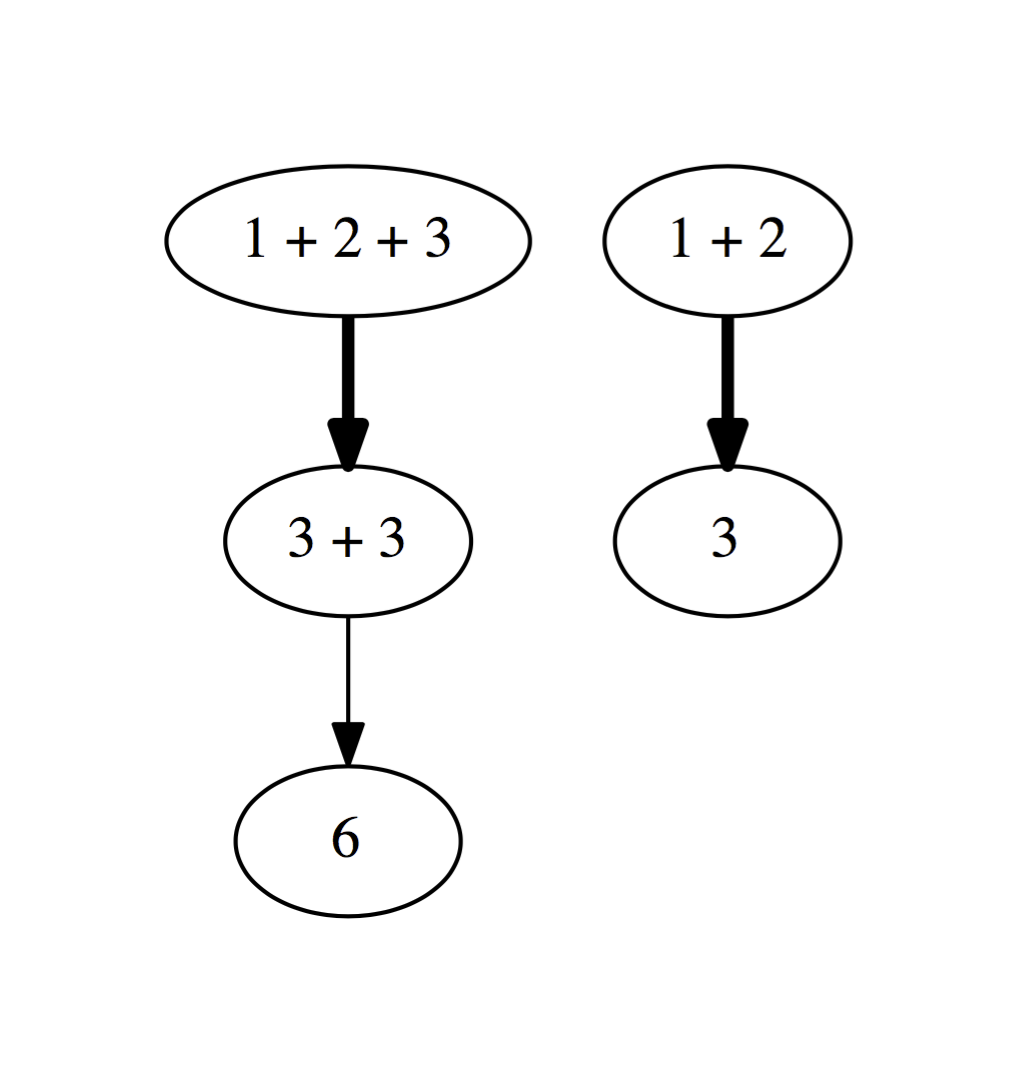
\includegraphics[height=2in]{simple.png}
  \caption{The reduction graph for \texttt{1+2+3}. The two edges
    produced by the transition from \texttt{1+2+3} to \hbox{\texttt{3+3}}
    are highlighted.}
\label{fig:simple-reduction-hi}
\end{figure}
%
Notice that when we transition from @1+2+3@ to @3+3@ we collect
both that edge \emph{and} an edge from the sub-term @1+2@ to @3@.
%
These additional edges allow us to implement two common debugging
operations \emph{post-hoc}: ``step into'' to zoom in on a specific
function call, and ``step over'' to skip over an uninteresting
sub-computation.

\paragraph{Interacting with the graph}
The reduction graph is useful for formulating and executing traversals,
but displaying it all at once would quickly become overwhelming.
%
Our interaction begins by displaying a big-step reduction, \ie the
witness followed by the stuck term.
%
The user can then progressively fill in the hidden steps of the
computation by selecting a visible term and choosing one of the
applicable traversal strategies --- described in
\S~\ref{sec:interactive} --- to insert another term into the
visualization.

\paragraph{Jump-compressed Witnesses}
It is rare for the initial state of the visualization to be
informative enough to diagnose the error.
%
Rather than abandon the user, we provide a short-cut to expand the witness
to a \emph{jump-compressed} trace, which contains every function call
and return step.
%
The jump-compressed trace abstracts the computation as a sequence of
call-response pairs, providing a high-level overview of steps taken
to reach the crash, and a high level of compression compared to the
full trace.
%
For example, the jump-compressed trace in Figure~\ref{fig:factorial}
contains 4 nodes compared to the 19 in the fully expanded trace.
%
Our benchmark suite of student programs shows that jump-compression is
practical, with an average jump-compressed trace size of 7 nodes and a
median of 5.

% A sample interaction with the trace of @fac 1@ can be seen in
% Figure~\ref{fig:nanomaly-factorial}.
% %
% % \begin{figure*}[t]
% % \centering
% % 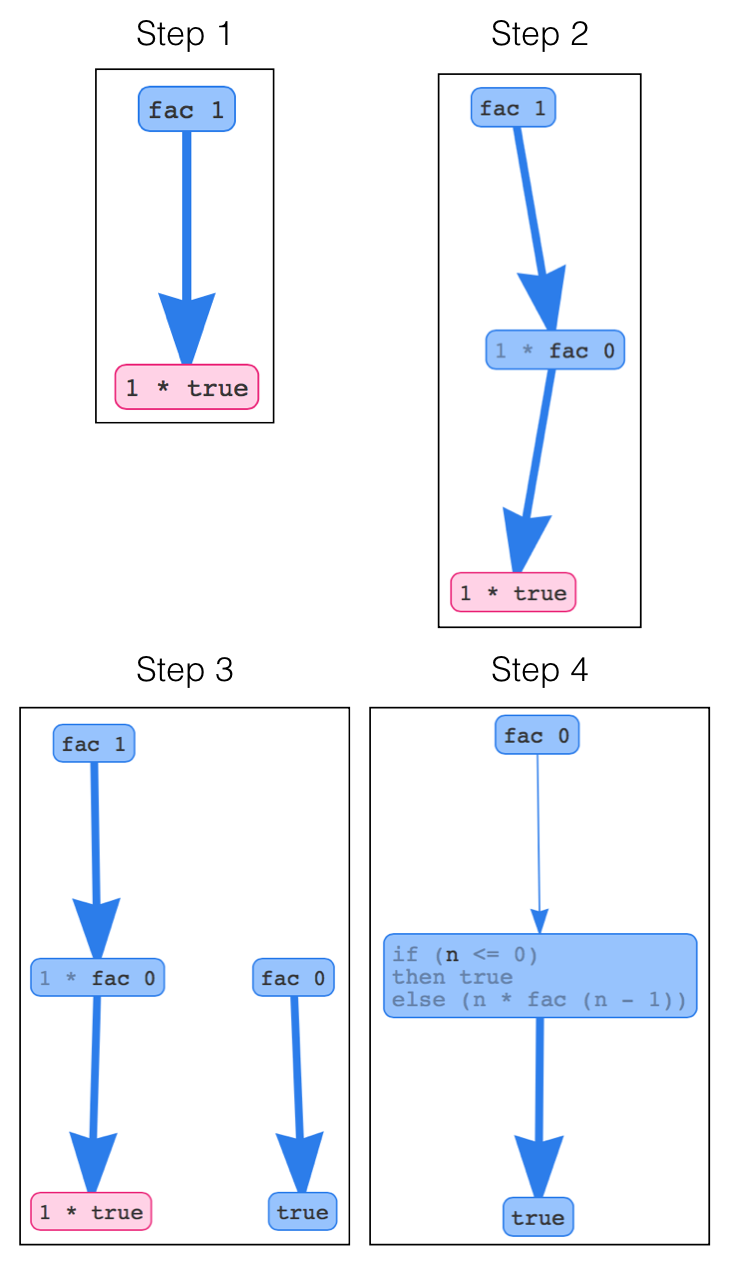
\includegraphics[width=0.8\linewidth]{fac-steps.png}
% % \caption{A sequence of interactions with the trace of
% %   \texttt{fac 1}. The stuck term is red, in each node the redex is
% %   highlighted. Thick arrows denote a multi-step transition, thin arrows
% %   denote a single-step transition. We start in step 1. In step 2 we jump
% %   forward from the witness to the next function call. In step 3 we step
% %   into the recursive \texttt{fac 0} call, which spawns a new ``thread''
% %   of execution. In step 4 we take a single step forward from
% %   \texttt{fac 0} (hiding the context for space).}
% % \label{fig:nanomaly-factorial}
% % \end{figure*}
% %
% The initial state of the visualization tells us that after some number
% of steps -- the thick arrow denotes a multi-step transition -- we try to
% multiply @1@ by @true@.

% Upon seeing the stuck term, we might wonder where @true@ came from.
% %
% To investigate we select the stuck term and click the ``jump backward''
% button to search backwards from the stuck term for the most recent
% function call, which brings us to @1 * fac 0@. Notice at this point that
% @fac 0@ is highlighted while @1 *@ is grayed out. This tells us that
% @fac 0@ is the redex in this term.

% @fac 0@ seems like the right thing to do so we choose to ``step into''
% it, which inserts a new multi-step transition from @fac 0@ to @true@.
% %
% Finally, we take a ``step forward'' from \hbox{@fac 0@,} bringing us to @fac@'s
% body. If we mouse over the body term we will see a popup with the
% environment at this point, notably telling us that @n = 0@. At this point
% it is clear that @fac@ handles the @n <= 0@ case incorrectly and should
% instead return an @int@.

% Upon seeing the stuck term, one might wonder where the @function@
% came from.
% %
% To investigate we select the stuck term and click the ``jump backward''
% button to search backwards from the stuck term for the most recent
% function call, which brings us to @listReverse [] = w@, in the same
% context as before.
% %
% Uncontent with the explanation so far, we ``step forward'' twice from
% the @listReverse []@ term, bringing us to @helper [] = w@.
% %
% At this point it is clear that the @helper@ function is not defined
% correctly, we have supplied it with the single argument we expected and
% yet it still returned a @function@.

% The problem is that the @function@ keyword in \ocaml defines an
% anonymous function that takes a single argument and immediately does a
% case-analysis without giving the argument a name.
% %
% The solution is to replace @function@ with an explicit @match xs with@
% -- naming the value we wish to case-analyse.
% %
% After applying our fix, \nanomaly -- and more importantly \ocaml --
% decide that @listReverse@ is safe to run.
% \ES{these last few paragraphs probably belong in the overview}
%





%%% Local Variables:
%%% mode: latex
%%% TeX-master: "main"
%%% End:
